\chap{Der Roboter findet seinen Weg selbständig}\label{ch.line}

Stellen Sie sich Lagerhaus mit Roboterwagen vor, welche Gegenstände von einer zentralen Verteilstelle herbringen. Dazu werden Linien auf den Boden des Lagerhauses gezeichnet und die Roboter erhalten die Anweisung bestimmten Linien zu folgen, bis diese den Lagerplatz für den gewünschten Gegenstand erreichen. Um dies zu tun, muss der Roboter diese Linien erkennen können. Schreiben Sie ein Programm, welches den Roboter einer Linie auf dem Boden folgen lässt.

{\raggedleft \hfill Beispielprogramm \bu{follow-line.aesl}}

Die Aufgabe ''Einer-Linie-Folgen'' zeigt die Herausforderungen bei der Konstruktion von Robotern in der realen Welt auf. So kann es sein, dass die Linie zum Beispiel nicht perfekt gerade ist, Staub kann auf der Linie liegen und diese abdecken, Dreck führt eventuell dazu, dass ein Rad weniger schnell dreht, als das andere. Damit der Roboter der Linie folgen kann, benötigt er eine \emph{Steuereinheit}, die entscheidet, wie viel Leistung jeder Motor benötigt, abhängig von den Daten, die von den Sensoren geliefert werden.

\sect{Die Linie und der Roboter}

Um einer Linie zu folgen, benutzen wir die Bodensensoren (\cref{ch.moving}). Zur Erinnerung: diese Sensoren arbeiten durch das Aussenden von Infrarotlicht (unsichtbar für das menschliche Auge) und dem Messen des reflektierten Lichts. Falls der Boden von heller Farbe ist, wird der Sensor viel reflektiertes Licht wahrnehmen und das Ereignis \blksm{lots-of-light} wird ausgelöst. Somit brauchen wir eine dunkle Linie, die wenig Licht reflektiert und das Ereignis \blksm{little-light} auslöst. Das lässt sich einfach mit dem Aufmalen oder Ausdrucken einer schwarzen Linie oder mit dem Anbringen eines schwarzen Isolierklebebandes auf den Boden bewerkstelligen (\cref{fig.tape}). Das Isolierband muss breit genug sein, damit beide Bodensensoren die schwarze Fläche gleichzeitig erkennen können. Eine Breite von 5 Zentimetern ist auf jeden Fall ausreichend, um dem Isolierband folgen zu können, auch wenn die Breite ein wenig variiert.

\begin{figure}
\subfigure[Thymio folgt einer Linie aus Isolierband]%
{\label{fig.tape}%
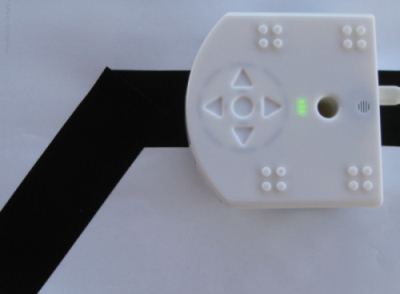
\includegraphics[height=0.35\textwidth]{blacktape}}
\hfill
\subfigure[Der linke Sensor ist neben und der rechte Sensor auf dem Isolierband
Der rote Punkt zeigt an, dass der linke Sensor viel reflektiertes Licht erkennt]%
{\label{fig.one-off}%
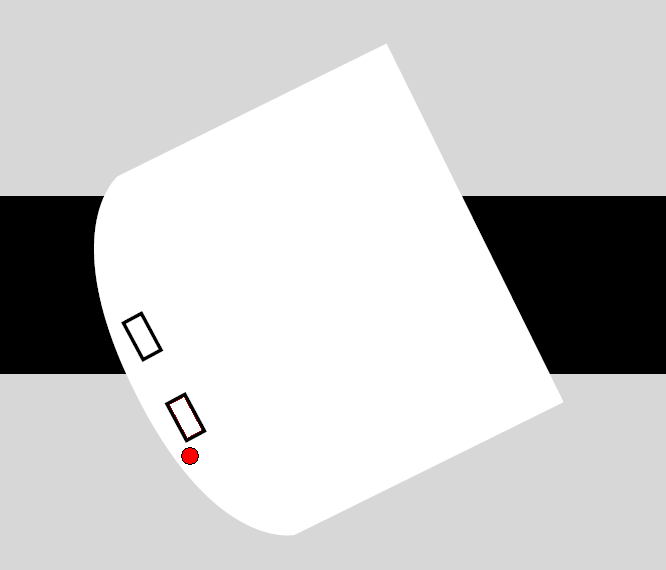
\includegraphics[height=0.35\textwidth]{thymio_half_on_line}}
\caption{Thymio auf dem Isolierband}
\end{figure}

Um ''Einer-Linie-folgen'' zu implementieren, bringen wir den Roboter zuerst dazu,  sich vorwärts zu bewegen, wenn \emph{beide} Sensoren eine dunkle Oberfläche erkennen (das schwarze Isolierband) und stoppen, falls \emph{beide} Sensoren die helle Oberfläche erkennen (nicht das Isolierband, sondern den hellen Boden bzw. Tisch). Die Ereignis-Aktions-Paare werden in der folgenden \cref{fig.start-stop} dargestellt.
                  
\begin{figure}
\subfigure[Starten und stoppen des Roboters]%
{\label{fig.start-stop}%
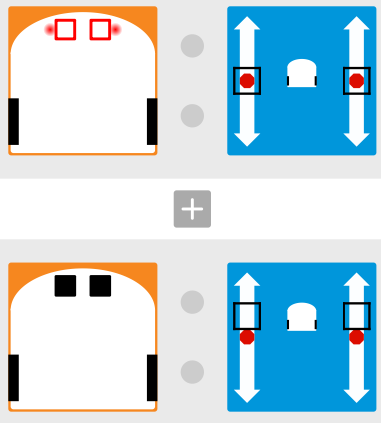
\includegraphics[width=0.45\textwidth]{line-forward}}
\hfill
\subfigure[Korrektur bei Abweichungen]%
{\label{fig.follow-line}%
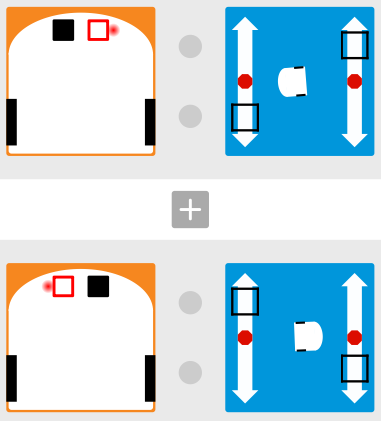
\includegraphics[width=0.45\textwidth]{line-controller}}
\caption{Programm ''Einer Linie Folgen''}\label{fig.follow-line-all}
\end{figure}

%\begin{center}
%\begin{tabular}{cc}
%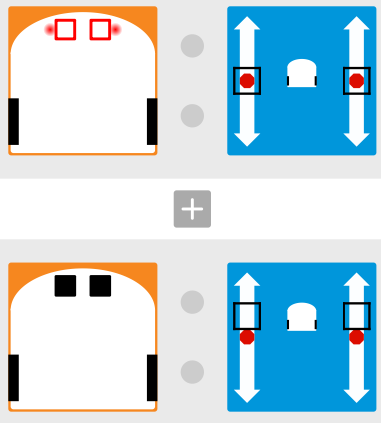
\includegraphics[width=0.4\textwidth]{line-forward} &
%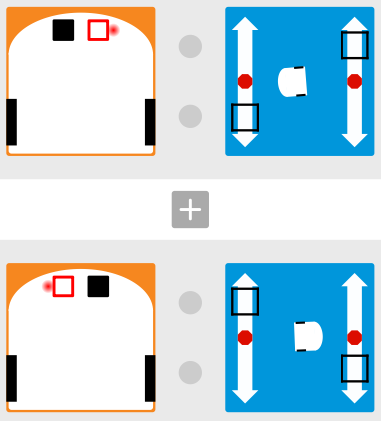
\includegraphics[width=0.4\textwidth]{line-controller} \\
%(a) Start and stop the robot & (b) Follow the line \\
%\end{tabular}
%\end{center}

\trickbox{Achten Sie darauf, ein USB-Kabel von ausreichender Länge zu verwenden (ca. 2m), damit Thymio trotz Bewegung mit dem Computer verbunden bleibt. Verlängerungskabel finden Sie in jedem Computershop. }

\informationbox{Wireless Thymio}{Falls Sie allerdings die neue Version von Thymio  besitzen, haben Sie beinahe unbegrenzte Bewegungsfreiheit. }
\sect{Ihre erste Steuerungseinheit}

Der nächste Schritt besteht im Programmieren der Steuerungseinheit,
die den Roboter der Linie folgen lässt. Wir benötigen wieder zwei Ereignis-Aktions-Paare (vgl. \cref{fig.follow-line}).

\begin{itemize}

\item Falls der Roboter nach der \emph{linken} Seite vom Isolierband abkommt, wird der \emph{linke} Sensor den hellen Boden erkennen, während der \emph{rechte} Sensor immer noch das dunkle Isolierband erkennt. In diesem Fall soll der Roboter ein wenig nach \emph{rechts} abbiegen.

\item Falls der Roboter nach der \emph{rechten} Seite vom Isolierband abkommt, wird der \emph{rechte} Sensor den Boden erkennen, während der \emph{linke} Sensor immer noch das dunkle Isolierband  erkennt. In diesem Fall soll der Roboter ein wenig nach \emph{links} abbiegen.

\end{itemize}

%Two event-actions pairs are needed, as shown in \cref{fig.follow-line}.

\sect{Einstellen der Parameter}

Es ist einfach zu erkennen, dass der Roboter nach rechts drehen muss, falls er von der linken Seite des Isolierbands abkommt, wie in \cref{fig.follow-line} dargestellt. Aber wie weit nach rechts soll er drehen? Falls die Drehung zu gering ausfällt, wird der rechte Sensor eventuell \emph{auch} vom Isolierband abkommen, bevor der Roboter auf die Spur zurückgelangt. Falls der Roboter jedoch zu stark nach rechts dreht, riskiert der Roboter die Isolierband-Spur auf der anderen Seite zu verlieren. In jedem Fall sind starke Drehungen gefährlich für den Roboter und jegliches Gut, das er transportiert.

Sie werden mit den Geschwindigkeiten des linken und rechten Motors experimentieren müssen, bis Sie \emph{zuverlässige} Werte finden. Zuverlässig heisst hier, dass der Roboter mit denselben Programmeinstellungen mehrmals erfolgreich der Linie folgt. Platzieren Sie bei jedem Versuch den Roboter ein wenig anders in Bezug auf Richtung und Position zum Isolierband.

Die Geschwindigkeit des Roboters auf dem Isolierband ist auch eine wichtiger Parameter. Ist der Roboter zu schnell, ist dieser schon vom Isolierband weggefahren, bevor die Drehbewegung die Richtung des Roboters verändern konnte. Ist der Roboter jedoch zu langsam, wird niemand Ihren Roboter kaufen um in einem Lagerhaus einzusetzen.

\exercisebox{\thechapter.1}{Der Roboter stoppt,	falls beide Sensoren erkennen, dass sie vom Isolierband abgekommen sind. Verändern Sie das Programm so, dass der Roboter eine leichte Drehung nach links vollführt mit der Absicht das Isolierband wiederzufinden. Versuchen Sie es auf einem Isolierband mit einer Linkskurve,	wie in der \cref{fig.tape} angezeigt. Versuchen Sie die Vorwärts-Geschwindigkeit des Roboters zu erhöhen. Was passiert, wenn der Roboter das Ende des Isolierbandes erreicht hat?}

\bigskip

\exercisebox{\thechapter.2}{Verändern Sie das Programm aus der vorangehenden Aufgabe so, dass der Roboter nach rechts dreht, falls er vom Isolierband abkommt. Was passiert? Es wäre wünschenswert, wenn der Roboter \emph{sich erinnern} könnte, welchen Sensor als letzter den Kontakt zum Isolierband verloren hat, um den Roboter in die korrekte Richtung zu führen und das Isolierband wieder zu finden. In \cref{ch.states} werden wir lernen, wie solche Informationen gespeichert werden.}

\bigskip

\exercisebox{\thechapter.3}{Experimentieren Sie mit unterschiedlichen Arten von Linien bzw. Anordnungen des Isolierbandes:
	\begin{itemize}[noitemsep,nosep,leftmargin=*]
		\item weite Kurven
		\item enge Kurven
		\item Zickzack-Linien
		\item breitere Linien (benutzen Sie dazu die doppelte Isolierbandbreite)
		\item schmälere Linien (schneiden Sie dazu das Isolierband in zwei Teile)
	\end{itemize}
	Veranstalten Sie mit Freunden ein Roboterrennen: Welcher Roboter folgt erfolgreich den meisten Linien? Welcher Roboter fährt am schnellsten eine Linie ab?}

\newpage

\exercisebox{\thechapter.4}{Diskutieren Sie den Effekt der folgenden Veränderungen auf den Thymio Roboter und dessen Fähigkeit der Linie zu folgen.
	\begin{itemize}[noitemsep,nosep,leftmargin=*]
		\item Die Messereignisse der Bodensensoren erfolgen öfters bzw. weniger oft als 10 Mal pro Sekunde.
		\item Die Sensoren sind weiter auseinander bzw. näher beisammen.
		\item Es gibt mehr als zwei Bodensensoren an der Unterseite des Roboters.
	\end{itemize}}
